\section{Generating Clusters}
Clusters were generated by sampling from a Gaussian distribution, and transforming the samples of each cluster based on the cluster's mean and covariance matrix. The random samples of a standard two-variable Gaussian distribution were generated using MATLAB's $randn()$ function. The samples were then transformed as shown by the example in MATLAB's documentation for $randn()$. The example provided shows how to transform a given vector, $\underbar{x}$, by the equation
\begin{eqnarray}
\label{eqn:chol_transform}
\underbar {y} = chol(\Sigma) \underbar {x} + \underbar {$\mu$}
\end{eqnarray}

where $\underbar{x}$ is a vector in the original space, $\underbar{y}$ is the transformed vector in the new space, and $chol(\Sigma)$ returns the Cholesky factorization of $\Sigma$.

Unit standard deviation contours were also created for each cluster. To find these contours, a vector of points that represented the unit standard deviation contour of a standard two-variable Gaussian distribution was transformed using the previously described transformation method for each cluster.

This method was confirmed as a viable method for transforming the data by using a second transformation to derive the unit standard deviation contours. The orthonormal covariance transformation shows that vectors of a Gaussian distribution with covarance $\Sigma$ can be transformed to have a covariance of I. This transformation is given by the equation
\begin{eqnarray}
\label{eqn:ortho_transform}
\underbar{x} = {\Lambda}^{-1/2} \Phi^T \underbar{y}
\end{eqnarray}

where columns of $\Phi$ are the eigenvectors of $\Sigma$ and the diagonal elements of $\Lambda$ are the eigenvectors of $\Sigma$. Taking the inverse of this equation and adding the specified mean results in the second transformation for deriving unit standard deviation contours:
\begin{eqnarray}
\label{eqn:ortho_inv_transform}
\underbar{y} = {(\Phi^{T})}^{-1} \Lambda^{1/2}\underbar{x}+\underbar{$\mu$}
\end{eqnarray}

Both transformations produced the same unit standard deviation contours, thus indicating the validity of the method used in this lab.

Visually, the unit standard deviation contours are centered on where the cluster data has the greatest density and shaped depending on the direction of the data distribution. By its definition, the unit standard deviation contour will contain approximately 78.2\% of the sample data.
 
 \subsection{Classes A and B}
 The two classes A and B are characterized by:

\begin{eqnarray}
{\mu}_{A}=\left[ \begin{smallmatrix} 5&10 \end{smallmatrix}\right]^{T} \; & {\Sigma}_{A}=\left[ \begin{smallmatrix} 8&0 \\ 0&4 \end{smallmatrix}\right] \nonumber\\
{\mu}_{B}=\left[ \begin{smallmatrix} 10&15 \end{smallmatrix}\right]^{T} \; & {\Sigma}_{B}=\left[ \begin{smallmatrix} 8&0 \\ 0&4 \end{smallmatrix}\right] \nonumber
\end{eqnarray}

\begin{figure}[ht]
\centering
	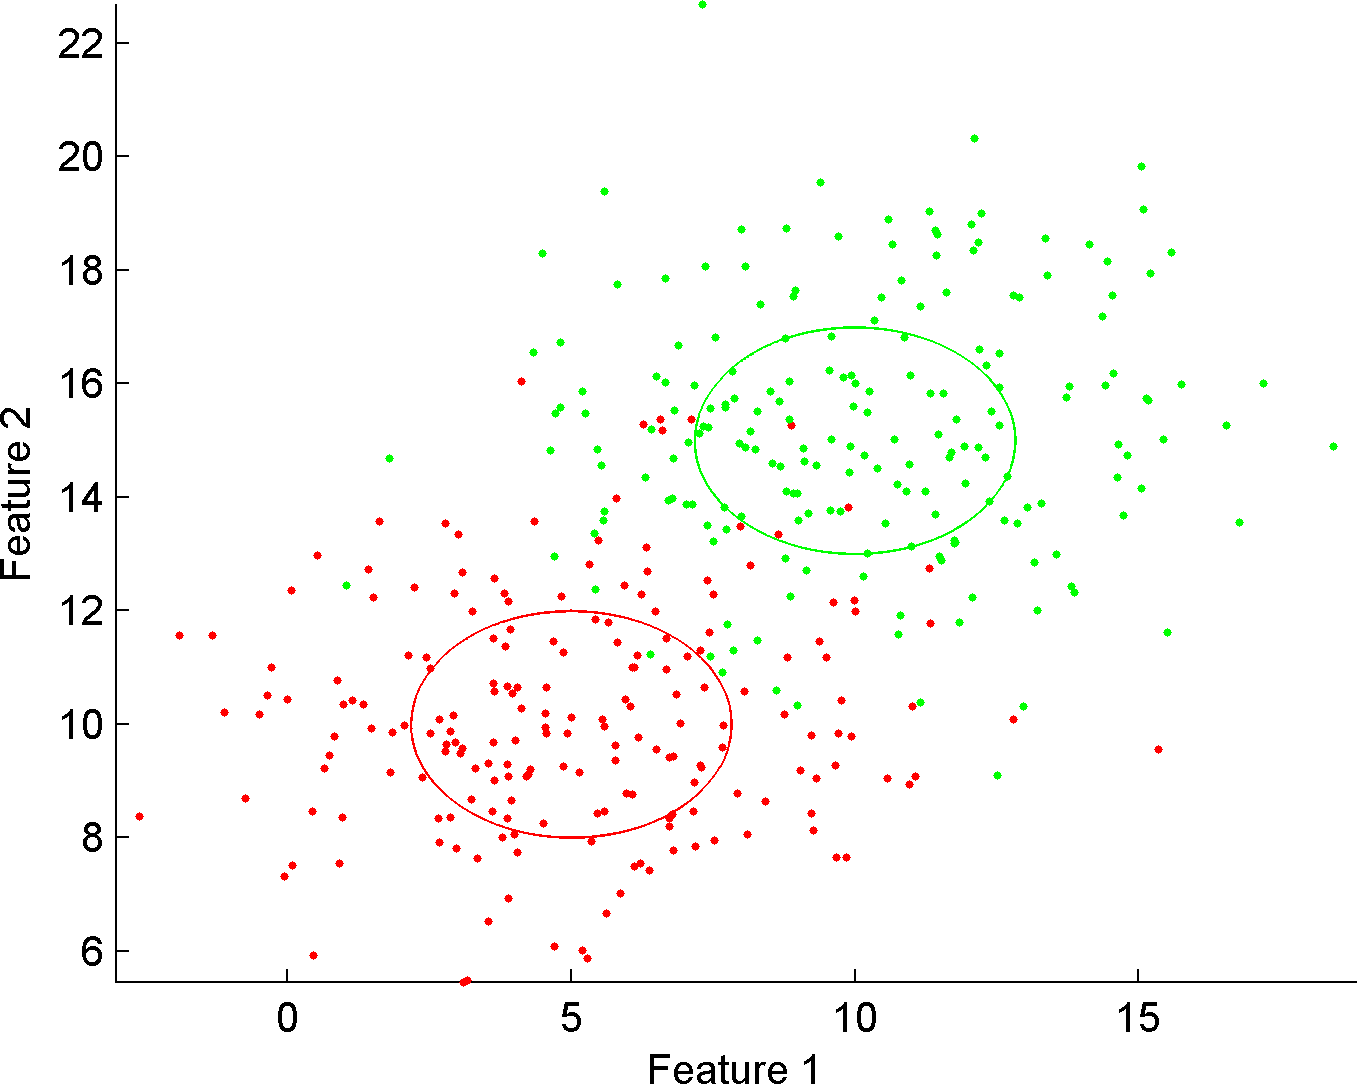
\includegraphics[width=0.9\linewidth]{fig1a-AB_cluster}
	\label{fig:clustersDataAB}
	\caption{Clusters A and B and their unit standard deviation contours}
\end{figure}

 \subsection{Classes C, D, E}
 The three classes C, D and E are characterized by:
 
 \begin{eqnarray}
{\mu}_{C}=\left[ \begin{smallmatrix} 5&10 \end{smallmatrix}\right]^{T} \; & {\Sigma}_{C}=\left[ \begin{smallmatrix} 8&4 \\ 4&40 \end{smallmatrix}\right] \nonumber\\
{\mu}_{D}=\left[ \begin{smallmatrix} 15&10 \end{smallmatrix}\right]^{T} \; & {\Sigma}_{D}=\left[ \begin{smallmatrix} 8&0 \\ 0&8 \end{smallmatrix}\right] \nonumber\\
{\mu}_{E}=\left[ \begin{smallmatrix} 10&5 \end{smallmatrix}\right]^{T} \; & {\Sigma}_{E}=\left[ \begin{smallmatrix} 10&-5 \\ -5&20 \end{smallmatrix}\right] \nonumber
\end{eqnarray}
 
 
\begin{figure}[ht]
\centering
	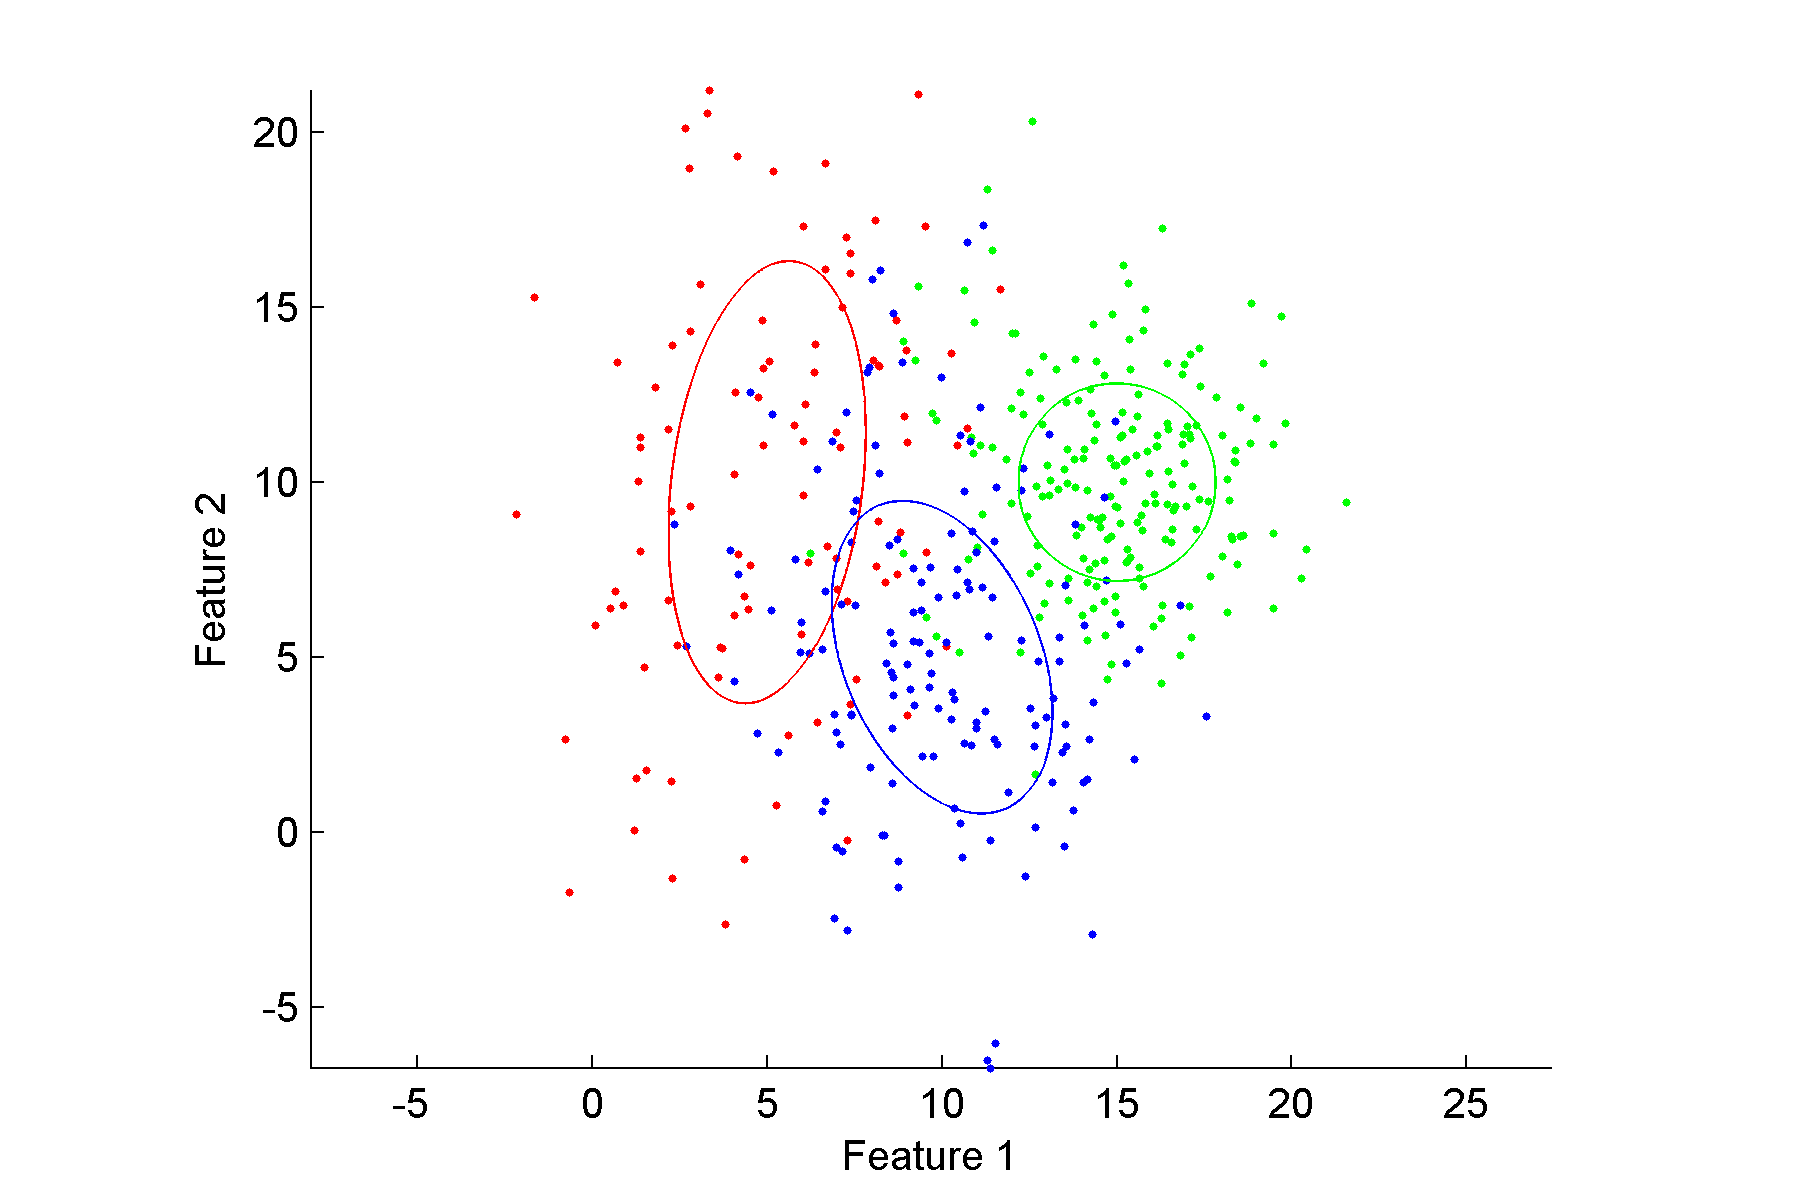
\includegraphics[width=0.9\linewidth]{fig1b-CDE_cluster}
	\label{fig:clustersDataCDE}
	\caption{Clusters C, D, and E and their unit standard deviation contours}
\end{figure}
 
\clearpage
